\vspace{10pt}
\section{Part 3: Cursor Trajectory Reconstruction and Error Analysis}

This part performs a reaching analysis by simulating the movement of a cursor based on velocity data (Part 2) and comparing it to a desired cursor position.
Because the MCI system operates with velocity control, it is necessary to integrate in time the velocities along the two axes to obtain the respective positions. The reconstructed trajectories are then compared with the ones registered during the experiment to evaluate the reconstruction error.

\subsection{Reaching Analysis Code Overview} 

 The code initializes position arrays for two methods: one for the custom algorithm (denoted as 'ours') and one for the Minimum Jerk Control (MCI) method. 
 First, the screen boundaries are defined with \texttt{screenCm} and the target apparitions by \texttt{spawnT}.  
 Then, two trajectories are reconstructed to determine the cursor positions: these are defined by \texttt{posOurs}, which was obtained using the activation envelopes from Part 1, and \texttt{posMCI}, obtained using the envelopes registered by the MCI system. Both start from the initial position of the cursor registered during the experiment (\texttt{cursorCmD}). Then a loop is built to perform three operations:
 \begin{itemize}
    \item Position update, using the relation \begin{equation}
                                                p(k) = p(k-1) + v(k) \cdot dt
                                              \end{equation}
          which is based on velocity. This is done at each sample.
    \item Clipping control, to clip to the screen between [0 0] (top left             screen position) and the boundaries defined by \texttt{screenCm}, so        to ensure that the cursor positions stay within the screen                  boundaries. 
    \item if resetAtEachTarget is true (reset condition) the positions are            reset to the desired cursor position at the current time step. This         allows to limit the integration error accumulation at the single            phase of target reach.
\end{itemize} 

Finally, after the loop, the code calculates the error between the simulated positions and the desired positions for both methods and prints the mean cursor error for each trajectory (registered and reconstructed) storing them in the  \texttt{errOurs} and \texttt{errMCI} variables. This is done through the function \texttt{vecnorm}. 

Then, before the animation part, the target coordinates are converted from pixels to cm. This conversion uses the physical dimensions of the screen and its pixel resolution, obtaining the matrix \texttt{targCm} which contains the target coordinates expressed in cm. This procedure allows to represent targets and cursor trajectories using the same unit of measurement, facilitating the graphical comparison.

Here an image of the cursor animation relative to the last instant of simulation and the mean cursor error are shown: 

\begin{figure}[H]
        \centering
        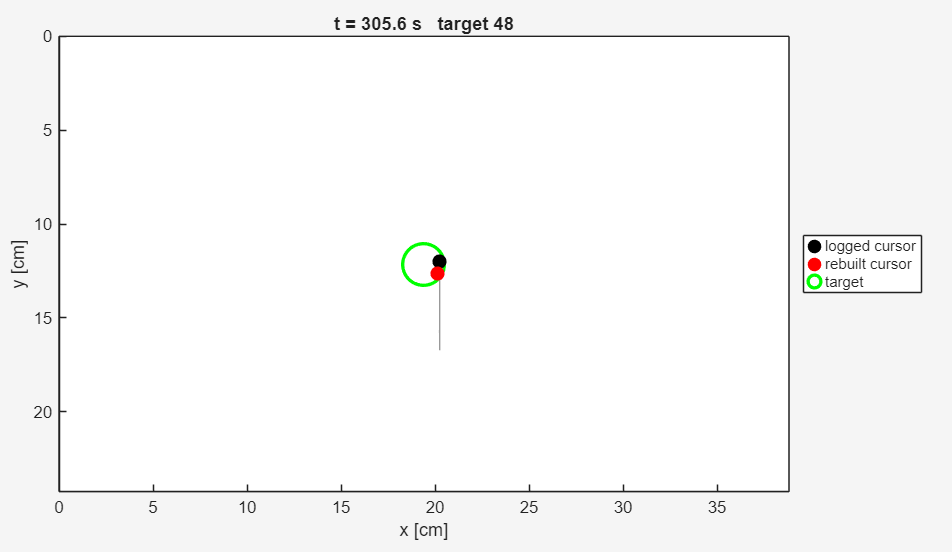
\includegraphics[width=\textwidth]{Images/Our data/cursor animation.png}
        \caption{Reconstructed and registered cursor positions, with the relative target, at the simulation last instant of time (t=305.6s, target no.48)
        }
\end{figure}

Mean cursor error: ours = 1.942 cm, MCI = 0.486 cm

During the entire animation time the simulation shows that the reconstructed cursor (red) is close to the logged cursor (black), indicating good agreement between the two positions. However, a small discrepancy is still present, highlighting that the reconstructed trajectory does not perfectly reproduce the original one.

By analyzing the mean cursor error, the results show that the reconstruction based on the original MCI envelopes is approximately four times more accurate than the one obtained using our preprocessing pipeline, even though the envelopes produced in Part 1 are similar to the original ones. This difference may be attributed to discrepancies in the envelope extraction process, particularly due to filtering and normalization, as well as the different temporal characteristics of offline and real-time processing. Moreover, \texttt{filtfilt} produecs envelopes without phase delay, while the MCI system works in real time and so it has an intrinsic delay.
